\section{Message Passing Framework}
\label{sec:algorithm}
\label{sec:receiver-structure}

In this section, we develop a message-passing (MP) framework
\cite{cai2026} based on the combined use of the sum-product rule and the
expectation propagation (EP) algorithm \cite{minka2001}. The framework interprets
the message updates on the factor graph in Fig.~\ref{fig:receiver-structure}
as iterations between two modules, namely, a linear estimator and a
joint denoiser. The linear estimator separately estimates each column of
$\mathbf X$ (i.e., $\mathbf x_j$) by exploiting the likelihood
$p(\mathbf y_j\mid\mathbf x_j)$ and the messages from the joint denoiser.
The joint denoiser estimates each device block $\mathbf X_k$ by exploiting
the priors $q_{\rm tr}(\mathbf H_k)$ and $p(\alpha_k)$, along with the
messages from the linear estimator.

\begin{figure}[!t]
\centering
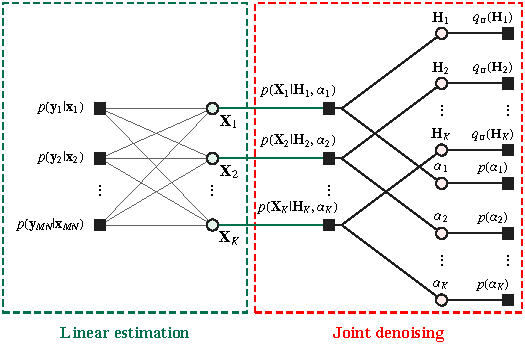
\includegraphics[width=\linewidth]{factor_graph.pdf}
\caption{Factor graph of \eqref{eq:working-posterior} using device blocks
$\mathbf X_k$ as variable nodes. Each likelihood factor depends on the corresponding
column entries from all device blocks. Circles and squares denote
variables and factors. The channel and activity prior branches are
adapted from \cite{cai2026}.}
\label{fig:receiver-structure}
\end{figure}

\subsection{Linear Estimation}
\label{sec:linear-estimation}

Following Turbo-CS \cite{ma2015}, we start by expressing the message to
the factor node $p(\mathbf y_j\mid\mathbf x_j)$ as
$\CN(\mathbf x_j;\mathbf x_j^{\rm pri},\gamma\I_{KN})$, where
$\mathbf x_j^{\rm pri}$ is the $j$th column of $\mathbf X^{\rm pri}$
and $\gamma>0$. Combining this message with the likelihood
$p(\mathbf y_j\mid\mathbf x_j)$ gives a Gaussian belief whose mean
and covariance are given by \cite{ma2017}:
\begin{align}
 \mathbf X_{\rm L}
 &=\mathbf X^{\rm pri}
 +\gamma\widehat{\mathbf A}^{\mathsf H}
 (\widehat\sigma^2\I_Q+\gamma\widehat{\mathbf A}\widehat{\mathbf A}^{\mathsf H})^{-1}
 (\mathbf Y-\widehat{\mathbf A}\mathbf X^{\rm pri}),
 \label{eq:linear-mean}\\
 \bm\Sigma_{\rm L}
 &=(\gamma^{-1}\I_{KN}+\widehat\sigma^{-2}\widehat{\mathbf A}^{\mathsf H}\widehat{\mathbf A})^{-1}.
 \label{eq:linear-variance}
\end{align}
Eqns.~\eqref{eq:linear-mean} and \eqref{eq:linear-variance} give, respectively,
the posterior mean matrix and per-column covariance from the linear MMSE
(LMMSE) estimator of $\mathbf X$. We further approximate the
covariance matrix using a shared scalar variance
$t_{\rm L}=\tr(\bm\Sigma_{\rm L})/(KN)$, resulting in a belief of the form
$\CN(\mathbf x_j;\mathbf x_{{\rm L},j},t_{\rm L}\I_{KN})$, where
$\mathbf x_{{\rm L},j}$ is the $j$th column of $\mathbf X_{\rm L}$.

The extrinsic message is proportional to the ratio of the above Gaussian
belief to the prior message. The variance $v_{\rm L}$ and mean matrix
$\mathbf R_{\rm L}$ are respectively given by
\begin{align}
 v_{\rm L}&=(t_{\rm L}^{-1}-\gamma^{-1})^{-1},
 \label{eq:linear-extrinsic}\\
 \mathbf R_{\rm L}&=v_{\rm L}
 \left(\frac{\mathbf X_{\rm L}}{t_{\rm L}}
       -\frac{\mathbf X^{\rm pri}}{\gamma}\right).
 \label{eq:linear-extrinsic-mean}
\end{align}
The extrinsic message flows rightward through the factor graph unchanged,
serving as the input to the joint denoiser, with $\mathbf R_k$ denoting the $k$th
device block of $\mathbf R_{\rm L}$ and $v=v_{\rm L}$.

\subsection{Joint Channel Estimation and Activity Detection}
\label{sec:joint-denoising}

For device $k$, the Gaussian message from the linear estimator,
with mean $\mathbf R_k$ and variance $v$, gives the local observation model
\begin{equation}
 \begin{gathered}
 \mathbf R_k=\alpha_k \mathbf H_k+\mathbf W_k,\\
 \vect(\mathbf W_k)\sim\CN(\mathbf0,v\I_D),
 \end{gathered}
 \label{eq:pseudo-awgn}
\end{equation}
where $\mathbf H_k\sim q_{\rm tr}$ and $D=MN^2$.

\subsubsection{Channel Estimation}
\label{sec:channel-estimation}

Under the active hypothesis $\alpha_k=1$, the Gaussian message
from the linear estimator has the form of the likelihood
$p(\mathbf R_k\mid\mathbf H_k,\alpha_k=1)$ in the AWGN model
\eqref{eq:pseudo-awgn}. Computing the conditional mean of $\mathbf H_k$
therefore amounts to MMSE denoising. The channel mean and a shared
average variance are approximated by
\begin{align}
 \mathbf F_k&\approx
 \E[\mathbf H_k\mid\mathbf R_k,\alpha_k=1],
 \label{eq:conditional-channel-integrals}\\
 \tau^{\rm post}&\approx\frac1{KD}\sum_{k=1}^K\tr\operatorname{Cov}
 (\vect(\mathbf H_k)\mid\mathbf R_k,\alpha_k=1).
 \label{eq:conditional-channel-variance}
\end{align}
Calculating the channel mean and shared average variance involves
high-dimensional integrals.

We approximate the channel prior by a Gaussian site
$\CN(\vect(\mathbf H_k);\vect(\mathbf E_k),\tau_k^{\rm ext}\I_D)$
\cite{vehtari2020}. Dividing the Gaussian belief,
with mean $\mathbf F_k$ and variance $\tau^{\rm post}$, by the input
likelihood gives the site parameters
\begin{align}
 \tau_k^{\rm ext}&=((\tau^{\rm post})^{-1}-v^{-1})^{-1},
 \label{eq:site-update}\\
 \mathbf E_k&=\tau_k^{\rm ext}\left(\frac{\mathbf F_k}{\tau^{\rm post}}-\frac{\mathbf R_k}{v}\right).
 \label{eq:site-mean}
\end{align}

\subsubsection{Activity Detection}
\label{sec:activity-detection}

Marginalizing over $\mathbf H_k$ in \eqref{eq:pseudo-awgn} yields the
likelihoods conditioned on $\alpha_k=1$ and $\alpha_k=0$, respectively:
\begin{align}
 q_{1,v}(\mathbf R)&=\E[\CN(\vect(\mathbf R);\vect(\mathbf H),v\I_D)],
 \label{eq:query-densities}\\
 q_{0,v}(\mathbf R)&=\CN(\vect(\mathbf R);\mathbf0,v\I_D).
 \label{eq:inactive-density}
\end{align}
The expectation is taken over $\mathbf H\sim q_{\rm tr}$.

The belief of $\alpha_k$ given $\mathbf R_k$ is a Bernoulli distribution
with parameter $p^\star(\mathbf R_k,v)$, where
\begin{equation}
 p^\star(\mathbf R,v)=\frac{\rho q_{1,v}(\mathbf R)}
 {(1-\rho)q_{0,v}(\mathbf R)+\rho q_{1,v}(\mathbf R)}.
 \label{eq:local-activity}
\end{equation}
We denote the approximation to $p^\star(\mathbf R_k,v)$ used in joint
estimation by $p_k$.

\subsubsection{Joint Estimation and Extrinsic Message}
\label{sec:joint-extrinsic}

Combining the site with the current Gaussian likelihood gives the
conditional channel variance and mean:
\begin{align}
 t_k&=\frac{\tau_k^{\rm ext}v}{\tau_k^{\rm ext}+v},
 \label{eq:conditional-moments}\\
 \mathbf H_k^{\rm post}&=\frac{\tau_k^{\rm ext}\mathbf R_k+v\mathbf E_k}{\tau_k^{\rm ext}+v}.
 \label{eq:conditional-channel-mean}
\end{align}

The approximate belief of $\mathbf X_k=\alpha_k\mathbf H_k$ is a
Bernoulli--Gaussian pdf \cite{liu2018}, with activity probability $p_k$
and a Gaussian active-channel component having mean
$\mathbf H_k^{\rm post}$ and covariance $t_k\I_D$.
The Gaussian projection gives the mean of $\mathbf X_k$ with respect
to the belief as
\begin{equation}
 \widehat{\mathbf X}_k=p_k\mathbf H_k^{\rm post}.
 \label{eq:mixture}
\end{equation}
The variances of the elements of $\mathbf X_k$ with respect to the belief
are averaged over all devices and channel coefficients to obtain
\begin{equation}
 \overline t_X=\frac1K\sum_k\left[
 p_kt_k+p_k(1-p_k)\frac{\norm{\mathbf H_k^{\rm post}}_F^2}{D}\right].
 \label{eq:joint-average-variance}
\end{equation}
Based on the above, the projected Gaussian belief is expressed as
$\CN(\vect(\mathbf X_k);\vect(\widehat{\mathbf X}_k),\overline t_X\I_D)$.

Finally, we calculate the message from the factor node
$p(\mathbf X_k\mid\mathbf H_k,\alpha_k)$ to the variable node
$\mathbf X_k$ as the ratio of the projected Gaussian belief to the
Gaussian message from the linear estimator. With $b=\overline t_X/v$, the extrinsic
variance and mean are respectively given by
\begin{align}
 \gamma_{\rm out}&=\frac{vb}{1-b},
 \label{eq:nonlinear-extrinsic}\\
 \mathbf X_{k,\rm out}&=\frac{\widehat{\mathbf X}_k-b\mathbf R_k}{1-b}.
 \label{eq:nonlinear-extrinsic-mean}
\end{align}
The extrinsic message in
\eqref{eq:nonlinear-extrinsic}--\eqref{eq:nonlinear-extrinsic-mean}
flows leftward through the factor graph unchanged, serving as the prior
message of the linear estimator in the next iteration, i.e.,
$\mathbf X^{\rm pri}=[\mathbf X_{1,\rm out}^{\mathsf T},\ldots,
\mathbf X_{K,\rm out}^{\mathsf T}]^{\mathsf T}$ and
$\gamma=\gamma_{\rm out}$.
